\documentclass[usenames,dvipsnames]{homework}
\usepackage{cancel}
\usepackage{amsthm}
\usepackage{cleveref}
\usepackage{upgreek}
\usepackage{mathrsfs}
\usepackage{tikz}
\usepackage{units}
%\usepackage{slashbox}
\usepackage{multirow}
\usepackage{listings}
\usepackage{bashful}
%\RequirePackage[usenames,dvipsnames]{color}

\lstloadlanguages{R}

\DeclareMathOperator{\cov}{cov}

\title{Kevin Joyce}
\course{Stat 542 - Sampling - Homework 4}
\author{Kevin Joyce}
\docdate{17 November 2014}
\begin{document} 
\newcommand{\figref}[1]{\figurename~\ref{#1}}
\renewcommand{\bar}{\overline}
\renewcommand{\hat}{\widehat}
\renewcommand{\SS}{\mathcal S}
\newcommand{\HH}{\mathscr H}
\newcommand{\mom}{\widetilde}
\newcommand{\mle}{\widehat \Uptheta}
\newcommand{\eps}{\varepsilon}
\newcommand{\todist}{\stackrel{D}\longrightarrow}
\newcommand{\iid}{\stackrel{\mathrm{iid}}\sim}
\newcommand{\toprob}{\stackrel{p}\longrightarrow} \newcommand{\TTheta}{\overline{\underline \Theta} }
\newcommand{\del}{\partial}
\newcommand{\approxsim}{\overset{\cdotp}{\underset{\cdotp}{\sim}}}
\newcommand{\RSS}{\ensuremath{\mathrm{RSS}}}
\newcommand{\MSE}{\ensuremath{\mathrm{MSE}}}
\newcommand{\SE}{\ensuremath{\mathrm{SE}}}
\newcommand{\SD}{\ensuremath{\mathrm{SD}}}
\newcommand{\TSS}{\ensuremath{\mathrm{TSS}}}
\newcommand{\Var}{\ensuremath{\mathrm{Var}}}
\newcommand{\Cov}{\ensuremath{\mathrm{Cov}}}
\newcommand{\SSReg}{\ensuremath{\mathrm{SSReg}}}
\renewcommand{\a}[1]{{\color{red} \it #1}}

\begin{longproblem} Consider the resutls from our in-class penny sampling project.  The sampling plans were:
  \begin{itemize}
    \item SRS: Zor, Vernon
    \item Double sampling, every 2nd: Eli and Guedem, Kevin and Lia
    \item Double sampling, every 4nd: Caitlin and Mike, Ann and Jacob
    \item Double sampling, every 5nd: Grant and Jon
  \end{itemize}

  The resulting seven data sets are given in the \texttt{R} script file \texttt{PennyData.R} on the course web page.  The data have been entered in the same format as for the biomass example on page 129 of the class notes:  the vector \texttt{y} contains the $n$ actual counts, the first $n$ elements of the vector \texttt{x} are the visual estimates corresponding to the actual counts, and the remaining elements of \texttt{x} are the visual counts for all 90 jars which is used only in part (c) below.

\subproblem{ For each of the seven sets of data above, estimate the total number of pennies in the population of 80 jars, and give the corresponding SE.  For the first two sets, the unbiased SRS estimator should be used.  For the latter five sets of data, a ratio estimator with double sampling should be used (using only the visual estimates in \texttt{x}). Show your work for just your own data set -- you do not need to show me the calculations for all seven sets of data. A table with the estimates and SE's would make a nice visual summary.  
}

\begin{solution}
For the simple random samples, we use the standard SRS estimates of the total
$$
\hat\tau = \frac Nn \sum_{i=1}^n y_i,\quad \hat{\Var}(\hat\tau) = \frac{(N-n)}{n-1}\sum_{i=1}^n (y_i - \bar y)^2.
$$
For each sample with a visual estimate, we estimate using a double-sampling estimator 
$$
\hat\tau_d = \left( \sum_{i=1}^n y_i \middle/ \sum_{i=1}^n x_i \right) \frac N{n'} \sum_{i=1}^{n'}x_i
$$
whose variance can be estimated by
$$
\hat{\Var}(\hat\tau_d)  = N(N-n')\frac {s^2}{n'} + N^2\left(1-\frac n{n'}\right) \frac{s_r^2}{n}
$$
where the $s^2/n'$ and $s_r^2/n$ are respective estimates of the variance of the total visual estimate and the ratio of the true estimate to the total and $n$ is the number actual counts and $n'$ is the number of visual estimates. The results are summarized below.

\begin{center}
\renewcommand{\arraystretch}{1.6}
\begin{tabular}{l|l r r }
       &  n   &$\hat\tau_r$&$\SE(\hat\tau_r)$ \\\hline
Zor    & 20   &  4768.00 & 348.90 \\
Vernon & 22   &  4090.91 & 294.24 \\
\end{tabular}
\begin{tabular}{l|l l r r}
		 & $n$& $n'$&$\hat\tau_{d} $&$\SE(\hat\tau_d)$ \\\hline
Eli and Guedem   & 21 & 42  &  3619.33   &   220.94 \\ 
Kevin and Lia    & 20 & 40  &  4067.64   &   205.50 \\
Caitlin and Mike & 17 & 68  &  3968.58   &   135.71 \\
Ann and Jacob    & 17 & 65  &  3796.83   &   162.63 \\
Grant and Jon    & 11 & 51  &  3929.41   &   449.15 \\\hline
\end{tabular}
\end{center}
\end{solution}

\subproblem{ Keeping in mind that the sampling effort (in terms of time) was roughly the same for all four sampling schemes, what, if anything, can you say about which method was most effective and why? Which group wins the dubious title of ``Least efficient estimators?'' Which group was most efficient?  Write a well-constructed paragraph or two to address this question. 
}
\begin{solution}
  In terms of estimated standard errors, Caitlin and Mike have the most
  efficient estimator. Moreover, it appears that a 4 to 1 ratio of visual to
  actual most efficiently extracts information since the other group with that
  plan, Ann and Jacob, also have a signficantly lower standard error than the
  others. Least efficient is Grant and Jon's group with a 5 to 1 ratio. 
  
  In terms of sampling effort, we can parametrize the variance of the estimator
  in terms of the ratio of the effort put toward visual and actual estimates.
  At one extreme, all effort goes to actual estimates which Zor and Vernon's plan.
  Note that their standard errors are nearly the largest.  As we include
  visual estimates at a 2 to 1 ratio, both of those groups have improved
  efficiency. Then the best estimators, at a 4 to 1 ratio. The group at the 5
  to 1 level had the largest standard error. Assuming all things equal,
  this group should have the most estimates, and it could be that standard
  error of the visual estimates dominates the standard error of the ratio estimator.
  
  However, note that the 5 to 1 group actually has a \emph{lower} number of visual estimates than those at the 4
  to 1 ratio, which indicates that either their visual estimator or actual
  estimator (or both) was slower than the corresponding 4 to 1 ratio groups. 
  It could be that
  extra effort (time) expended by the visual estimator that did not contribute
  useful information to the estimate, hence less total information and a less
  efficient estimate.
\end{solution} 

\subproblem{ Just to see how much difference it makes, for the five double sampling schemes, calculate the ratio estimate and SE of the total number of pennies using the visual estimates for all 80 jars (\texttt{x.all}), as in Chapter 7.  Does using all 80 visual estimates reduce the corresponding SE's from part (a) much?
}
\begin{solution}
\begin{center}
\renewcommand{\arraystretch}{1.6}
\begin{tabular}{l|l l r r r r}
		 & $n$& $n'$&$\hat\tau_{d}$&$\SE(\hat\tau_d)$&$\hat\tau_r $&$\SE(\hat\tau_r)$\\\hline
Kevin and Lia    & 20 & 40  &  4067.64     &   205.50        &   3976.48   &    109.93\\
Caitlin and Mike & 17 & 68  &  3968.58     &   135.71        &   4068.67   &    118.68\\
Ann and Jacob    & 17 & 65  &  3796.83     &   162.63        &   3732.92   &    130.02\\
Grant and Jon    & 11 & 51  &  3929.41     &   449.15        &   4030.00   &    418.97\\\hline
\end{tabular}
\end{center}

It appears that the reduction in the standard error increases with the addition of more estimates, as expected.  That is, the 2 to 1 group added 40 estimates and reduced the standard error by nearly 100, whereas the 4 to 1 groups experienced a less dramatic decrease in the standard error with the addition of 12 to 15 estimates.  
\end{solution}

\subproblem{ Some of the ``actual'' counts were off -- most by 1 or 2, but in two instances by 10.  I replaced these mistaken counts by the true counts so that we could make a fairer comparison of the sampling methods.  But suppose, I had retained the incorrect actual counts. More generally, suppose there was significant random measurement error in the actual counts.  How would that affect estimates and SE's?  (Think about what would happen to the regression and to $s_r^2$.)
}

\begin{solution}
  If we model this with some random component added to the response, say $y_i + \eps_i$. If $E\eps_i \not=0$, it is clear, that this will introduce a bias in the estimates.
  
Even if $E\eps_i = 0$, it will still have an effect on both terms of the linearized variance of the ratio estimator  
$$
\Var(\hat\tau_d)  = N(N-n')\sigma^2 + N^2\left(1-\frac n{n'}\right)\sigma_r^2. 
$$
which is now a random quantity depending on $\eps_i$. If we take the expected value, $\sigma^2$ increases since $E(y_i+\eps_i - \mu)^2 > (y_i - \mu)^2$. Similarly, $\sigma_r^2$, which is a measure of the discrepancy between $y_i$ and $R x_i$, increases with the addition of $\eps_i$.  That is, measurement error degrades the efficiency of the estimators.

\end{solution}

\subproblem{ Estimate the optimal sampling ratio $n/n'$ by using estimates of $\sigma_r^2$ and $\sigma^2$ from any one of the double sampling data sets (tell me which one you used).  Use three different estimates of the cost ratio $c'/c$; a `best guest' based on your experience in the classroom and a smaller value and a bigger value.
}

\begin{solution}
  For a given cost ratio $c'/c$ of visual estimates to actual estimate, the optimal ratio of actual estimates to visual estimates in terms  
  $$
  \frac{n}{n'} = \sqrt{\frac{c'}{c} \left(\frac{\sigma_r}{\sigma^2 - \sigma_r^2}\right)}.
  $$
  Using Caitlin and Mike's data to estimate $\sigma_r^2$ and $\sigma^2$, we obtain
\begin{center}
\renewcommand{\arraystretch}{1.6}
\begin{tabular}{l|c c c }
$c'/c$ &$\frac 15$&$\frac 13$&$\frac 12$\\
$n/n'$ & 0.176    & 0.227    &0.278     \\
\end{tabular}
\end{center}
So, if the true cost ratio is between $1/2$ and $1/3$, the plan for their group was nearly optimal with $n/n' = .25$.
\end{solution}
\end{longproblem}
\newpage
%%%%%%%%%%%%%%%%%%%%%%%%%%%%%%%%%%%%%%%%%%%%%%%%%%%%%%%%%%%%%%%%%%%%%%%%%%%%%%%%
%                               Problem 2 
%%%%%%%%%%%%%%%%%%%%%%%%%%%%%%%%%%%%%%%%%%%%%%%%%%%%%%%%%%%%%%%%%%%%%%%%%%%%%%%%
\problem{ For this problem, you will need to retrieve the data file \texttt{fraser.txt} from the course web page.  This files contains the mean monthly flows ($m^3/\text{sec}$) of the Fraser River at Hope, B.C.~ from March 1912 through December 2012 (100+ years, 1210 observations). These data are in the text file \texttt{fraser.txt}.  A function called \texttt{systematic} can also be found on the web page and is required for this problem.  
}

\subproblem{ Plot the flows over time: use the command \texttt{ts.plot(x)} (time series plot).  It may be hard to see patterns since a lot of data (1210 flows) is compressed into the plot.  To get around this, you might plot just the first 250 observations by \texttt{ts.plot(x[1:250])} or any other subset of the data by using \texttt{ts.plot(x[a:b])}.  Describe any patterns you see in a few sentences. (You do not need to include the plots. )
}

\subproblem{ Consider the 1210 monthly flows as the population and suppose that you want to estimate the mean of the mean monthly flows for this period from  a sample of months.  Compare systematic sampling (with random starting point) with intervals of 3, 6, 9, 11, 12, 13, 23, 24 to each other and to simple random samples (SRS's) of the same sample sizes.  Do this by computing the theoretical standard deviations of the estimators (you can use the function \texttt{systematic} as discussed below).  Discuss your results.  Are the results what you would expect?  How big an effect can matching the data pattern have on the systematic estimator?  How do the systematic SE's compare to those for SRS of the same sample size?
}

Note: For a systematic sample with interval $k$, there are only $k$ possible samples corresponding to the $k$ possible starting points.  The sampling distribution of the mean therefore contains only $k$ equally likely values and the theoretical variance of the estimator can be easily computed.  The function \texttt{systematic(x,k)} automates this; it computes the expected value and standard deviation of the samling distribution of the sample mean based on a systematic sample with interval $k$ (with random starting point) form the population vector \texttt{x}.

\begin{solution}
  \begin{minipage}{.45\textwidth}
    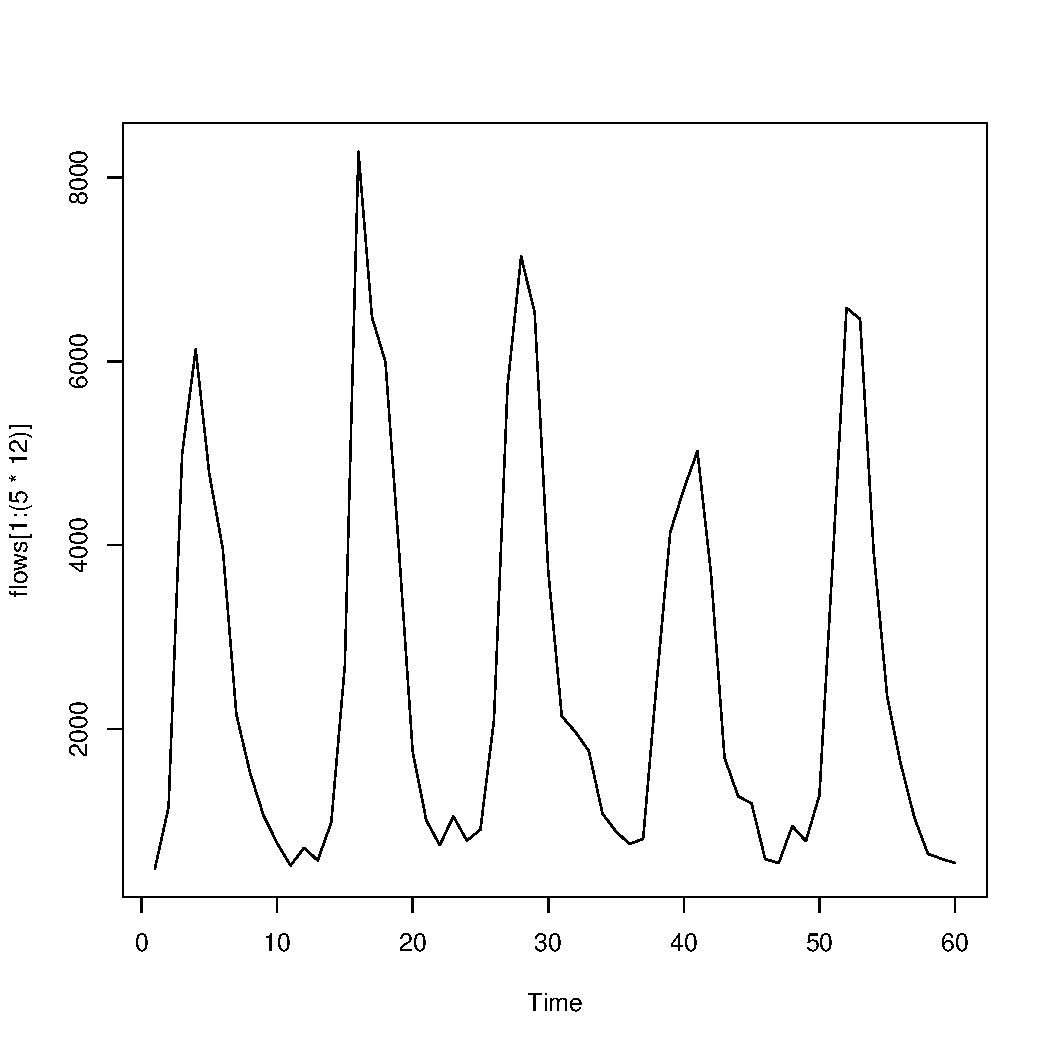
\includegraphics[width=\textwidth]{fraser_flow.pdf}
  \end{minipage}
  \begin{minipage}{.45\textwidth}
    In the plot to the left, we plot the first 5 years of monthly flows.  Note that the
    flow oscillates with a frequency of about twelve months with varying amplitude. 
    This oscillation will
    be problematic for a systematic sample whose period is nearly the same as
    the flow frequency as shown in the following analysis.
  \end{minipage}

In the following table, we take compute every systematic sample of a given size $k$, and compute their expected value and standard deviation.
\begin{center}
{\small
\renewcommand{\arraystretch}{1.6}
\begin{tabular}{l|r r r r r r r r}
$k$		&         3  &       6  &      9   &      11  &    12   &      13  &      23  &      24\\ \hline
$E(\bar y_k)$   &  2708.86 & 2708.99 & 2709.11 & 2708.96 & 2705.99 & 2708.94 & 2709.24 & 2705.68\\
$\SD(\bar y_k)$ &   138.06 &  \a{958.17} &  150.09 &  121.96 & \a{2070.48} &   82.10 &  135.27 & \a{2025.50}\\
$n$	        &   403    &  201    &  134    &  110    &  100    &   93    &   52    &   50   \\
\end{tabular}
}
\end{center}

Note that systematic samples that repeat every $6$th, $12$th, and $24$th month have
very large standard deviations.  This is due to the yearly cycle
of the flows.  For the annually and biannually systematic samples, responses
will be consistently tight around the randomly chosen first value, since they
match the river's natural cycle, and the standard
error is approximately the amplitude of the oscillation. That is, if your
random starting time to  measure is in the Spring, you will estimate a high
flow, whereas if you randomly choose Winter, you will estimate a low flow, but
in both cases only be measuring one yearly point on the annual cycle.
Similarly in the six month systematic sample, you only measure two yearly points.
So, it's not surprising it's standard error is nearly half that of the 12 and 24 month samples.

In the following table, an SRS was conducted and the theoretical standard error is calculated
based on the the complete data.  Note that these do not consistently out-perform the systematic
samples, but do not suffer from the occasionally huge standard deviation.
\begin{center}
{\small
\begin{tabular}{l|r r r r r r r r}
$k$		&         3  &       6  &      9   &      11  &    12   &      13  &      23  &      24\\ \hline
  $\bar y$	&2832.47 & 2638.06 & 2759.91 & 2693.88 & 3146.93 & 2283.13 & 2502.81 & 2321.98\\
$\SD(\bar y)$    &86.18  & 136.44  & 172.57  & 192.58  & 202.89  & 211.05  & 287.38  & 293.33 \\
$n$	        &   403      &  201    &  134    &  110      &  100    &    93    &    52    &    50   \\
\end{tabular}
}
\end{center}
\end{solution}

\problem{ In class, we discussed the following nonresponse example.  A survey is mailed to a random sample of 120 individuals in a population of 400 individuals.  30 out of the 120 people respond to the survey and of these 30, 20 respond ``Yes'' to some particular question of interest.  A followup telephone survey is done on a random sample of 25 of the 90 nonrespondents.  20 of the 25 respond to the phone survey; of these 20, 4 answer to the question of interest.  Ignoring the 5 who didn't respond even to the survey, estimate the proportion of all 400 individual in the population who would respond ``Yes'' to the question of interest and attach a standard error to this estimate.  Compare the estimate and SE to the estimate and SE we would get if we simply treated the total of 50 respondents as an SRS from the population.  }

\begin{solution}
  We poststratify the sample into responders and nonresponders of the first
survey, and estimate the proportion of the population that would or would not
respond to the initial survey by $n_h'/n'$ where $n_h'$ is the sample stratum
size  and $n'=120$ is the sample size.  Due to the non-response at the second level,
we also assume $n_2 = 20$ instead of 25. Let $\bar y_h$ be the positive response proportion,
then the resulting estimate is
$$
  \bar y_d = \sum_{h=1}^2 \left( \frac{n'_h}{n'} \right) \bar y_h = \left( \frac{30}{120} \right) \frac{20}{30} + \left(\frac{90}{120}\right)\frac{4}{20} \approx 0.317.
$$
The estimated standard error of the poststatification estimator is given by
$$
  \hat{\Var}(\bar y_d) = \left(\frac{N-1}{N}\right)\sum_{h=1}^2 \left(\frac{n_h'-1}{n'-1} - \frac{n_h-1}{N-1}\right) \left(\frac{n_h'}{n'}\right) \frac{s_h^2}{n_h} + \left[\frac{N - n'}{N(n'-1)}\right] \sum_{h=1}^2 \frac{n_h'}{n'} (\bar y_h - \bar y_d)^2
$$
where the within stratum sample variance is $ s_h^2 = \frac{n_h}{n_h-1}  \bar y_h(1-\bar y_h) $.
The resulting estimate for the standard error is
$$
  \SE(\bar y_d) \approx 0.0706 
$$
Had we just treated the responses as a simple random sample then we would estimate $\bar y_{srs} = \frac {24}{50} = .48$ with standard error 
$$
  \SE(\bar y_{srs}) = \sqrt{\left(1 - \frac nN\right) \bar y_{srs}(1-\bar y_{srs})/(n-1)} \approx 0.0668.
$$ 
Note the difference in these two estimators.  This is a result of weighting the the first-responders equally with the non-first-responders in the SRS, despite them being the majority of the population.  We note, however, that the reduction in standard error from stratifying (which is minimal when estimating proportions) is offset by estimating the population ratios $N_h/N$, hence the standard error of the post stratefied estimator is \emph{higher} than that of the SRS.

\end{solution}

\begin{longproblem} Two dentists A and B make a survey of the teeth of 200 children in a village.  Dr.~A selects an SRS of 20 children and counts the number of decayed teeth for each child, with the following results:
\begin{verbatim}
  0 0 0 0 0 0 0 0 1 1 1 1 2 2 3 3 4 5 9 10
\end{verbatim}
Dr.~B examines all 200 children, recording merely whether each child has any decayed teeth or not.  She finds 60 children have no decayed teeth.  

Give an estimate along with an SE for the total number of decayed teeth among all 200 children in the village,
\begin{enumerate}[(a)]
  \item using only A's results.
  \item using post-stratification of A's results by B's results.
\end{enumerate}

\begin{solution}
  Using the standard SRS estimator, we estimate
$$
\hat\tau_{SRS} = \frac Nn \sum_{i=1}^n y_i = 420\text{ teeth } ,\quad \SE(\hat\tau_{SRS}) = \sqrt{\frac{(N-n)}{n-1}\sum_{i=1}^n (y_i - \bar y)^2} \approx 125\text{ teeth. }
$$
Taking Doctor B's estimates as a secondary variable $x$ and using the poststratification estimator with known $\tau_x$, we estimate
$$
  \hat \tau_{pst} = \sum_{h=1}^2 N \left(\frac{N_h}{N}\right) \bar y_h = 490\text{ teeth}
$$
and we estimate the standard error using the variance estimate
$$
  \hat{\Var}(\hat \tau_{pst}) = \frac{N-n}n \sum_{h=1}^2 \left(\frac{N_h}{N} \right) \frac{s_h^2}{n_h} + \frac 1{n^2}\left(\frac{N-n}{N-1}\right) \sum_{h=1}^2 \frac{N-N_h}{N} \frac{s_h^2}{n_h}
$$
where $s_h^2$ is the within stratum sample variance.  This yields $\SE(\hat\tau_{pst}) \approx 110.84$.  We note that the second term, which accounts for the uncertainty of randomly sized sample strata, is generally ignored since it does not contribute much to the calculation.  If we do this, we obtain $\tilde{\SE}(\hat\tau_{pst}) \approx 109.7$ teeth.  The stratification offers a reasonable reduction in standard error.

\end{solution}
\end{longproblem}
\vspace{-2em}

\begin{longproblem}
  Andre McDonald, a student in this class some years ago, did a project to compare various sampling methods for estimating the total number of sweetclover shrubs in a square plot 108 feet on a side.  One of his methods was a line-intercept survey.  The resulting data is in the file \texttt{SweetCloverTransects.csv}.  It contains the ``widths'' (in inches, perpendicular to the transect) of the intercepted plants on each of 12 random parallel transects.  The transects are parallel to one pair of sides.  Note that there is no overlap data either within or between transects so that the ``separate transects'' estimates of the population total and SE must be used.
\begin{enumerate} 
  \item Estimate the total number of plants using the data from all 12 transects, calculate the SE and compute a \unit[95]{\%} confidence interval.
  \item How many transects would be required to estimate the total number of plants to within $\pm 100$ with \unit[95]{\%} probability.
\end{enumerate}

{\bf Solution:}

  Let $w=1296$ be the total width perpendicular to the transects in inches. Using the separate transect estimator for the total count ($y_i = 1$) $v_i = \sum \frac{1}{p_k} = \sum \frac{w_k}{w}$ where $w_k$ is the width of the intercepted plant on the $i$th transect. An unbiased estimate of the total is given by 
  $$
    \hat\tau_p = \frac 1n \sum_{i=1}^n v_i \approx 740
  $$
  with the standard error estimate
  $$
    \SE(\hat\tau_p) = \sqrt{\frac 1{n(n-1)} \sum_{i=1}^n (v_i - \hat\tau_p)^2} \approx 101
  $$
  A normal based \unit[95]{\%} confidence interval is given by $\hat\tau_p \pm q_{.975} \SE(\hat\tau_p) $ gives $\big(541.75,\, 937.69 \big) $.


  If we take the sample variance of $v_i$ to be the true variance, $\sigma_v^2$, of the estimator $\hat\tau_p$ and assume it is distributed normally, then a confidence interval with margin of error $d=100$ satisfies
  $$ 
  d^2 = q_{.975}^2 \frac{\sigma_v^2}{n} \implies n = \left(\frac d{q_{.975}}\right)^2 \sigma_v^2 \approx 47.03.
  $$
%  Note the lack of the finite population correction factor simplifies this formula.
\end{longproblem}

\vspace{-3em}
\problem{ {\it Thompson 16.3 Modified.} A simple random sample of $n=20$ of $N=100$ plots are selected for an aerial survey and the following numbers of moose are detected: 
$$ 
0,0,0,0,1,2,6,11,5,1,9,3,1,0,10,4,7,22,0,0,5.
$$
Assuming detectability of .89,} 

\subproblem{ estimate the mean number of moose and give an estimate the standard error of the estimator. }

\begin{solution}
Assuming that the detectability has no uncertainty, we use the unbiased SRS estimator
$$
  \hat\mu_1 = \frac{\bar y}{p} \approx \text{4.607 moose per plot}
$$
We estimate the standard error with
$$
\SE(\hat\tau_1) = \sqrt{\frac{1}{p^2} \left[
\left(\frac{N-n}{N}\right)\frac{s^2}{n} + \left(\frac{1-p}{N}\right)\bar y
\right]} \approx 1.256\text{ moose per plot. }
$$
Note that to obtain estimates for the total, we need only multiply these by 100.
\end{solution}

\subproblem{ Now suppose that the detection probability of $p=0.89$ was
estimated from another study independent of this one with a standard error of
$\SE(\hat p)$. Using the data given in problem 3, estimate the standard error
of the mean number of moose when $\SE(\hat p)$ is
$0.01,0.02,0.03,0.04,0.05,0.08$ and $0.10$ (note: you can do all these values
simultaneously in \texttt{R} by creating a vector of these values and using
this vector in the formula for the SE).  Write a couple of sentences comparing
the standard errors resulting form the different values for $\SE(\hat p)$. Does
the SE of the detection probability have much effect on the value of $\SE(\hat
p)$? 
}

\begin{solution}
The estimator $\hat\tau_2$ simply replaces $p$ with $\hat p$, and we obtain the same estimate.  When we include variability in estimating $\hat p$, a standard error estimate is
$$
  \tilde\SE(\tau_2) = 
\sqrt{\frac{1}{\hat p^2} \left[
\left(\frac{N-n}{N}\right)\frac{s^2}{n} + \left(\frac{1-\hat p}{\hat p}\right)\bar y
 + \frac{\bar y^2}{\hat p^2} \hat{\Var}(\hat p)\right]}
$$
A summary of the calculations with the given $\SE(\hat p)$ are given below
\begin{center}
  \renewcommand{\arraystretch}{1.4}
{
\begin{tabular}{l| r r r r r r r r r}
$\SE(\hat p)$   &   0.010 & 0.020 & 0.030 & 0.040 & 0.050 & 0.060 & 0.070 & 0.080 & 0.100\\\hline
$\SE(\hat\tau_2)$&  1.257 & 1.261 & 1.266 & 1.273 & 1.283 & 1.294 & 1.308 & 1.323 & 1.359\\
\end{tabular}
}
\end{center}
As expected, the standard error of $\hat\tau_2$ increases as $\SE(\hat p)$ does.  However, the overall effect on the additional variance from estimating $\hat p$ is dominated by the first two terms. 

\end{solution}

\problem{ Omitted }

\begin{longproblem} Problem 4 of Homework 3 was a two-stage sampling plan to estimate the average height of seedlings in a field.  Bootstrap this problem.  On each bootstrap replication, take a random sample with replacement of $n=5$ plots and then within each of the selected plots taking a random sample with replacement of the appropriate number of seedlings (which varies from plot to plot).  However, there are only 25 plots in the population so, at the first stage, do what is often suggested for finite population: create a bootstrap population of 5 copies of each of the 5 selected plots, then each bootstrap sample will consist of a sample of 5 without replacement from the bootstrap population.  At the second stage, just ignore the finite population (since \unit[10]{\%} is a relatively small proportion) and sample with replacement from the seedlings within a plot.  (If we wanted to take population size of each plot into account, it would be a little involved since the population size is not an even multiple of the sample size. So, for example, for plot 1, where there are 52 seedlings and a sample of size 5, the bootstrap population would consist of 10 copies of each seedling plus an 11th copy of the two of the seedlings, selected randomly.  Except that the 11th copies would not stay the same form bootstrap iteration to iteration: we would select them anew randomly on each iteration.) 

 You will have to program the bootstrap yourself.  At the end, you will have at least 10,000 bootstrapped values of your statistic.  Examine the sampling distribution of the estimate of the population mean, compute the bootstrap SE and compute the percentile confidence interval. Comment
\end{longproblem}
\vspace{-2em}
\begin{solution}
  \begin{minipage}{.45\textwidth}
    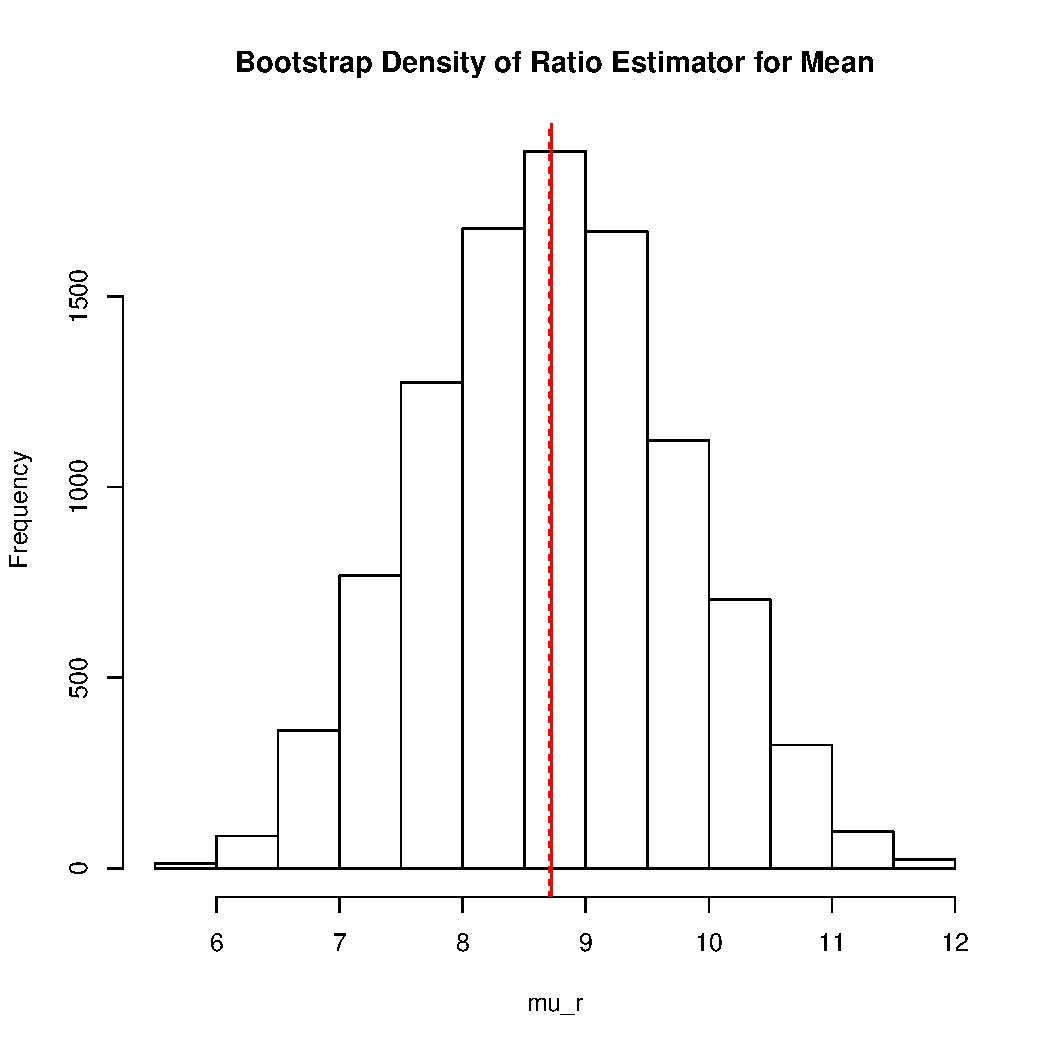
\includegraphics[width=\textwidth]{bootstrap.pdf}
  \end{minipage}
  \begin{minipage}{.45\textwidth}
    The bootstrap density appears to be fairly symmetric and is nearly centered at
    the estimated value (from homework 3) of $8.705$ inches (indicated by a
    dashed line to the left).  Although, there is evidence of the bias in the
    estimator, since the mean of the bootstrap density is $8.714$ inches
    (indicated by a solid line to the left).  The bootstrap standard error is
    $1.03$ inches while the linearized estimate was 1.11 inches.  These generally agree.
    The percentile confidence interval is
    $\big(6.23,\,10.73\big)$ inches. 
  \end{minipage}
\end{solution}
\newpage
\lstset {
	language=R,
	frame=shadowbox,
	basicstyle=\footnotesize\ttfamily, % the size of the fonts that are used for the code
  	backgroundcolor=\color{white},  % choose the background color. You must add \usepackage{color}
  	showspaces=false,               % show spaces adding particular underscores
  	showstringspaces=false,         % underline spaces within strings
  	showtabs=false,                 % show tabs within strings adding particular underscores
  	rulecolor=\color{black},        % if not set, the frame-color may be changed on line-breaks within not-black text (e.g. commens (green here))
  	tabsize=2,                      % sets default tabsize to 2 spaces
  	captionpos=b,                   % sets the caption-position to bottom
  	breaklines=true,                % sets automatic line breaking
  	breakatwhitespace=false,        % sets if automatic breaks should only happen at whitespace
  	keywordstyle=\color{RoyalBlue},      % keyword style
  	commentstyle=\color{YellowGreen},   % comment style
  	stringstyle=\color{ForestGreen}      % string literal style
	}
\begin{lstlisting}
> ################################################################################
> # Problem 1
> ################################################################################
... # Load SRS Data
> n = length(y) 
> tauhat = N * mean(y) 
> se.tauhat = N*sqrt((1-n/N)*var(y)/n)
> double_sample_estimate = function(x,y) { 
+   n <- length(y) 
+   x1 = x[1:n]
+   np <- length(x)
+   r <- sum(y)/sum(x1)
+   tau.hat.x <- (N/np)*sum(x)
+   tau.hat.r <- r*tau.hat.x
+   sr2 <- (1/(n-1))*sum((y-r*x1)^2)
+   var.tau.hat.r <- (N*(N-np)*var(y))/np + N^2*((np-n)/np)*sr2/n
+   se.tau.hat.r = sqrt(var.tau.hat.r)
+   return(
+     c(
+       'tau.hat.r'=tau.hat.r,
+       'se.tau.hat.r'=se.tau.hat.r
+     )
+   )
+ }
> ratio_estimate = function(x,y) { 
+   n <- length(y) 
+   tau.x <- sum(x)
+   x = x[1:n]
+   r <- sum(y)/sum(x)
+   tau.hat.r <- r*tau.x
+   sr2 <- (1/(n-1))*sum((y-r*x)^2)
+   var.tau.hat.r <- N^2*(1-n/N)*sr2/n
+   se.tau.hat.r = sqrt(var.tau.hat.r)
+   return(
+     c(
+       'tau.hat.r'=tau.hat.r,
+       'se.tau.hat.r'=se.tau.hat.r
+     )
+   )
+ }
... # Load and run functions on double sample data
> # part (e)
> # Use Caitlin and Mike
> y <- c(83,17,58,49,35,60,32,46,28,91,67,47,37,41,56,50,46) 
> cost_ratios = c(1/5,1/3,1/2) 
> n = length(y) 
> x = x[1:n] 
> r = sum(y)/sum(x) 
> sr2 <- (1/(n-1))*sum((y-r*x)^2) 
> s2 <- var(y) 
> (sample_ratio = sqrt(cost_ratios * sr2/(s2-sr2)))
[1] 0.1759690 0.2271750 0.2782314
> ################################################################################
> # Problem 2
> ################################################################################
> rm(list=ls()) 
> source('systematic.R') 
> flows = scan('fraser.txt')
Read 1210 items

> N = length(flows) 
> ts.plot(flows[1:(5*12)]) 
> dev.copy(pdf,'fraser_flow.pdf')
pdf 
  3 
> dev.off()
X11cairo 
       2 
> k = c(3,6,9,11,12,13,23,24) 
> systematic_samples = sapply(k, function(k){ systematic(flows,k) }) 
> (round(systematic_samples,2))
          [,1]    [,2]    [,3]    [,4]    [,5]    [,6]    [,7]    [,8]
evalue 2708.86 2708.99 2709.11 2708.96 2705.99 2708.94 2709.24 2705.68
stddev  138.06  958.17  150.09  121.96 2070.48   82.10  135.27 2025.50
n       403.00  201.00  134.00  110.00  100.00   93.00   52.00   50.00

> (n = floor(length(flows)/k))
[1] 403 201 134 110 100  93  52  50

> srs_flows = function(n){
+   samp = sample(flows,n)
+   c('y.bar'=mean(samp), 'se.y.bar='=sqrt((1-n/N)*var(flows)/n))
+ } 
> srs = sapply(n,srs_flows) 
> round(srs,2)
             [,1]    [,2]    [,3]    [,4]    [,5]    [,6]    [,7]    [,8]
y.bar     2798.00 2699.58 2603.88 2778.25 2763.31 2473.81 2960.48 2456.40
se.y.bar=   86.18  136.44  172.57  192.58  202.89  211.05  287.38  293.33
> ################################################################################
> # Problem 3
> ################################################################################
> rm(list=ls()) 
> N = 400 
> nhp = c(30,90) 
> nh = c(30,20) 
> ybar = c(20/30,4/20) 
> w = nhp/sum(nhp) 
> (ybar.d = sum(w*ybar))
[1] 0.3166667

> sh2.over.nh = ybar*(1-ybar)/(nh-1) 
> (
+   se.ybar.d = sqrt(
+     (N-1)/N * sum( ((nhp-1)/(sum(nhp)-1) - (nh-1)/(N-1)) * (w*sh2.over.nh) )
+     + (N - sum(nhp))/(N*(sum(nhp)-1)) * sum( nhp/sum(nhp) * (ybar - ybar.d)^2 )
+   )
+ )
[1] 0.07056032

> n = 50 
> (p = 24/n) 
[1] 0.48

> (se.p = sqrt((1-n/N) * p*(1-p)/(n-1)) )
[1] 0.06676184
> ################################################################################
> # Problem 4
> ################################################################################
> rm(list=ls()) 
> N = 200 
> y = c( 0, 0, 0, 0, 0,
+        0, 0, 0, 1, 1, 
+        1, 1, 2, 2, 3, 
+        3, 4, 5, 9, 10 ) 
> n = length(y) 
> # part (a)
> ( tau.srs = N * mean(y) )
[1] 420

> ( se.tau.srs = N*sqrt( (1 - n/N) * var(y)/n ) )
[1] 124.5708

> # part (b)
> x = y < 1 # x is true when if there is a decayed tooth 
> nh = table(x) # False comes first 
> Nh = c(200-60,60) 
> s2h = tapply(y,x,var) # estimate of sig^2_h 
> ( tau.post = sum(tapply(y,x,mean) * Nh) ) 
[1] 490

> var.term1 = N^2 * (1 - n/N)/n * sum( Nh/N * s2h ) 
> var.term2 = N^2 * 1/n^2 * (N-n)/(N-1) * sum( (N-Nh)/N * s2h ) 
> (se.tau.post.both.terms = sqrt(var.term1 + var.term2))
[1] 110.8436

> (se.tau.post.first.term = sqrt(var.term1))
[1] 109.6689
> ################################################################################
> # Problem 5
> ################################################################################
> clovers = read.csv('SweetCloverTransects.csv') 
> width = 108*12 # We take inches to be the units 
> y = tapply(clovers$width,clovers$transect,function(w) { sum(1/(w/width)) }) 
> ( v_st=mean(y) )
[1] 739.7165

> ( se.v_st=sqrt(var(y)/length(y)) )
[1] 101.0065

> ( ci.v_st = v_st + c(-1,1)*qnorm(.975)*se.v_st )
[1] 541.7475 937.6855

> # part (b)
> d = 100 
> (n_suff = (qnorm(.975)/d)^2*var(y) )
[1] 47.03007
> ################################################################################
> # Problem 6
> ################################################################################
> rm(list=ls()) 
> # part (a)
> N = 100 
> mooses = c( 0, 0, 0, 0,
+           1, 2, 6,11,
+           5, 1, 9, 3,
+           1, 0,10, 4,
+           7,22, 0, 0
+         )

> n = length(mooses) 
> p = .89 
> (muhat = mean(mooses)/p)
[1] 4.606742

> (var.srs = (1/p^2)*((N-n)/N) * var(mooses)/n)
[1] 1.572901

> (var.det = (1/p^2)*((1-p)/N) * mean(mooses))
[1] 0.005693726

> (se.muhat = sqrt(var.srs + var.det))
[1] 1.256421

> # part (b)
> se.p = c(1,2,3,4,5,6,7,8,10) / 100 

> var.phat = 1/p^2 * (mean(mooses)/p)^2 * se.p^2 
> se2.muhat = sqrt(var.srs + var.det + var.phat) 
> t(round(data.frame(
+    'se.p'     = se.p,
+    'se2.muhat' = se2.muhat
+    ),3))
           [,1]  [,2]  [,3]  [,4]  [,5]  [,6]  [,7]  [,8]  [,9]
se.p      0.010 0.020 0.030 0.040 0.050 0.060 0.070 0.080 0.100
se2.muhat 1.257 1.261 1.266 1.273 1.283 1.294 1.308 1.323 1.359
> ################################################################################
> # Problem 8
> ################################################################################
> rm(list=ls()) 

> seedlings = data.frame(
+ 'plot' = c(rep(1,5),rep(2,6),rep(3,6),rep(4,5),rep(5,5)),
+ 'height' = c( 12 , 11 , 11 , 10 , 13 ,    
+               10 ,  9 ,  7 ,  8 ,  8 , 10,
+                6 ,  5 ,  7 ,  5 ,  6 ,  4,
+                7 ,  8 ,  6 ,  7 ,  6 ,   
+               10 , 11 , 13 , 12 , 12 ))   

> N = 25                            # Total number of primary units

> Nh = c(52,56,60,46,49)            # Known secondary unit totals

> nh = table(seedlings$plot)  # Secondary sample sizes

> n = length(nh)                    # Primary sample size

> # This function does a two stage resample
> # where the first stage resamples without 
> # replacement from bootstrap population
> # made from replicating the sample (N/n) times
> # to correct for a small sampling population
> twostage.resample = function(y,factors,N,Nh) { 
+   factors = factor(factors)               # Make sure this is a factor level
+   stageone.pop = rep(1:n,N/n)             # Construct indices for bootsrp population 
+   stageone.idx = sample(stageone.pop,N/n)   # Sample WITHOUT replacement
+   ragged_table = tapply(y,factors,        # Create a list of strata for indexing
+                  function(yh){ yh })      #   using the first stage samples indices
+   stagetwo = function(yh) {               # Function for sampling second stage
+     sample(yh,replace=T)                  # Here we "could" implement a finite pop
+   }                                       # correction, but instead do the regular bootstrp
+  yy = lapply(ragged_table[stageone.idx]   # Sample the second stage
+             , stagetwo)                   # Using the stagetwo function
+  repidx = rep(stageone.idx,nh[stageone.idx])# Make a vector of indices 
+                                             # for making resampled factor and Nh
+  ffactors = levels(factors)[repidx]         # Make a vector of the factors sampled at 
+                                             # stage one
+  yy = unlist(yy,use.names=F)                # Change yy from a ragged list back to a vector
+
+  samp = data.frame(
+    'resampidx' = rep(1:n,nh[stageone.idx]),# Use this for the "new" strata index
+    'factors'   = ffactors,		     # The factor (plot#) that was resampled
+    'y'	 = yy,                       # The resampled value
+    'Nh'        = Nh[repidx]		     # The true strata size matched up with resample
+  )
+  return(samp)
}

> # This function is meant to work with
> # the naming convention in twostage.resample
> estimate.ybar = function(resampidx,Nh,y) {
+   NNh = tapply(Nh,resampidx,mean) # Reduce Nh to strata
+   ybarh = tapply(y,resampidx,mean)# Strata wise means
+   sum(NNh*ybarh)/sum(NNh)         # Ratio estimator
+ }

> boot = function() {
+   samp = twostage.resample(seedlings$height,seedlings$plot,N,Nh)
+   estimate.ybar(samp$resampidx,samp$Nh,samp$y)
+ }

> straps = replicate(10000,boot())
> mur = estimate.ybar(seedlings$plot,rep(Nh,nh),seedlings$height) 
> hist(straps, main="Bootstrap Density of Ratio Estimator for Mean", xlab="mu_r") 
> abline(v = mean(straps), lty='solid', col='red') 
> abline(v = mur, lty='dashed', col='red') 
> (muboot = mean(straps))
[1] 8.71367 

> (seboot = sd(straps))
[1] 1.025719

> sorted_straps = sort(straps) 
> (boot.ci = sorted_straps[c(50,9750)])
[1]  6.23026 10.73388
\end{lstlisting}

\end{document} 

